\question Alice and Bob are throwing baseballs and they want to see who can throw a baseball further. The distance Alice throws a baseball is modeled as a uniform distribution between $0$ and $5$ while the distance Bob throws a baseball is modeled as a uniform distribution between $0$ and $10$. Assume Alice and Bob throw independently, what is the probability that Bob's throw will be further than Alice's?
\begin{solution}
	Let $A \mathtt{\sim} U[0, 5]$ be the distance of Alice's throw and let \\
	$B \mathtt{\sim} U[0, 10]$ be the distance of Bob's throw.  \\
	We know the density of $A$ is $\frac{1}{5}$ and the density of $B$ is $\frac{1}{10}$ \\
	We can draw the following graph where $x$ is Alice's throw and $y$ is Bob's throw. \\
	
	\begin{center}
		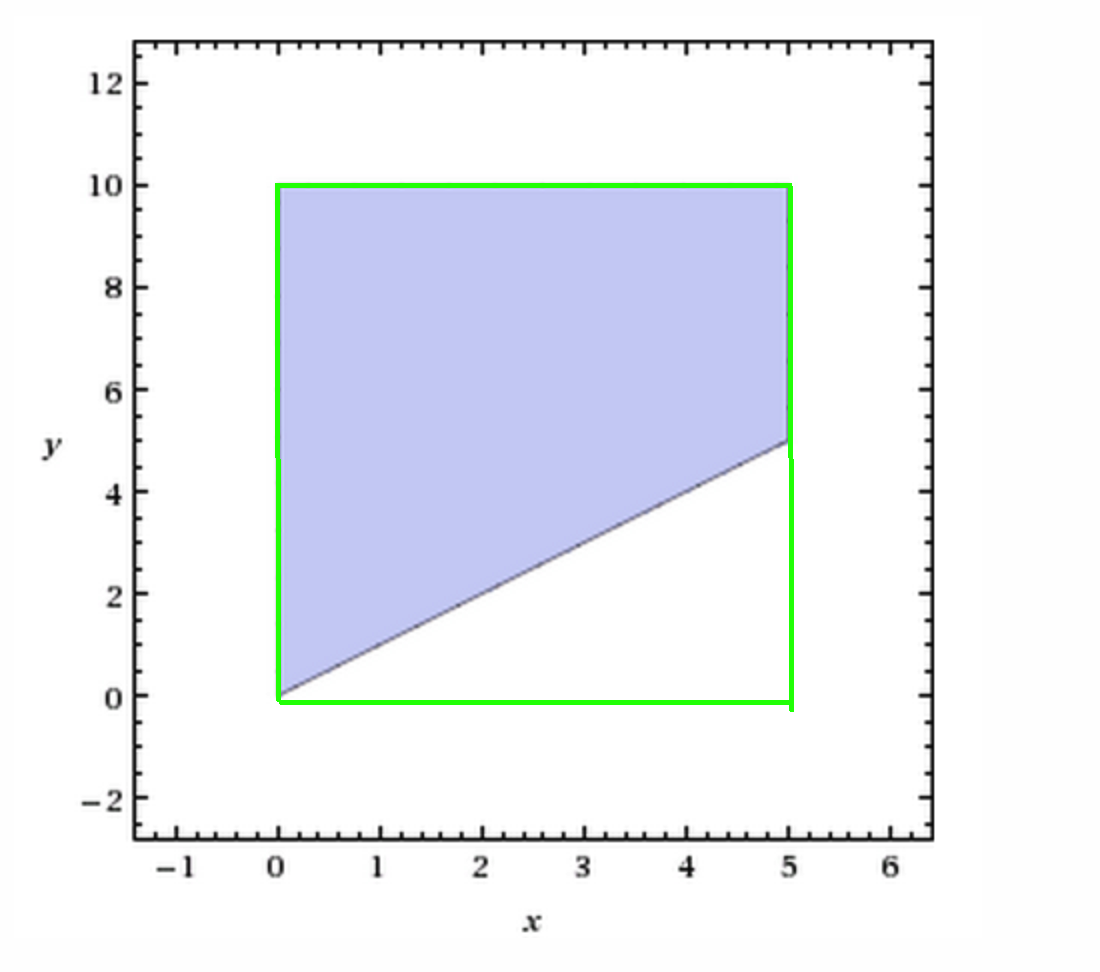
\includegraphics[width=5cm]{joint_uniform.png}
	\end{center}
	The green outline is the entire sample space while the shaded region is the region of interest. As we can see, the blue region takes up $\frac{3}{4}$ of the total sample space. \\
	
	A more algebraic approach is to use double integrals. \\
	We fix Alice's throw to be between $0$ and $5$ and we only consider Bob's throw if it is greater than Alice's. \\
	The joint pdf $f_{A, B} = f_A * f_B = \frac{1}{50}$ as $A$ and $B$ are independent.  \\
	Therefore, \\
	$P(B > A)   \\
	= \int\limits_{0}^{5}\int\limits_{a}^{10}f_{A, B} db da \\
	=  \int\limits_{0}^{5}\int\limits_{a}^{10}\frac{1}{50} db da \\
	= \int\limits_{0}^{5} (\frac{1}{50}b)\big|_{a}^{10} da \\
	=  \int\limits_{0}^{5} \frac{1}{5} - \frac{a}{50} da \\
	= (\frac{1}{5}a - \frac{a^2}{100})\big|_{0}^{5} = 1 - \frac{25}{100} = \frac{3}{4}$
	
\end{solution}